\section{Messergebnisse und Auswertung}
\subsection{Peltierelement}

\begin{figure}[H]
\begin{center}
  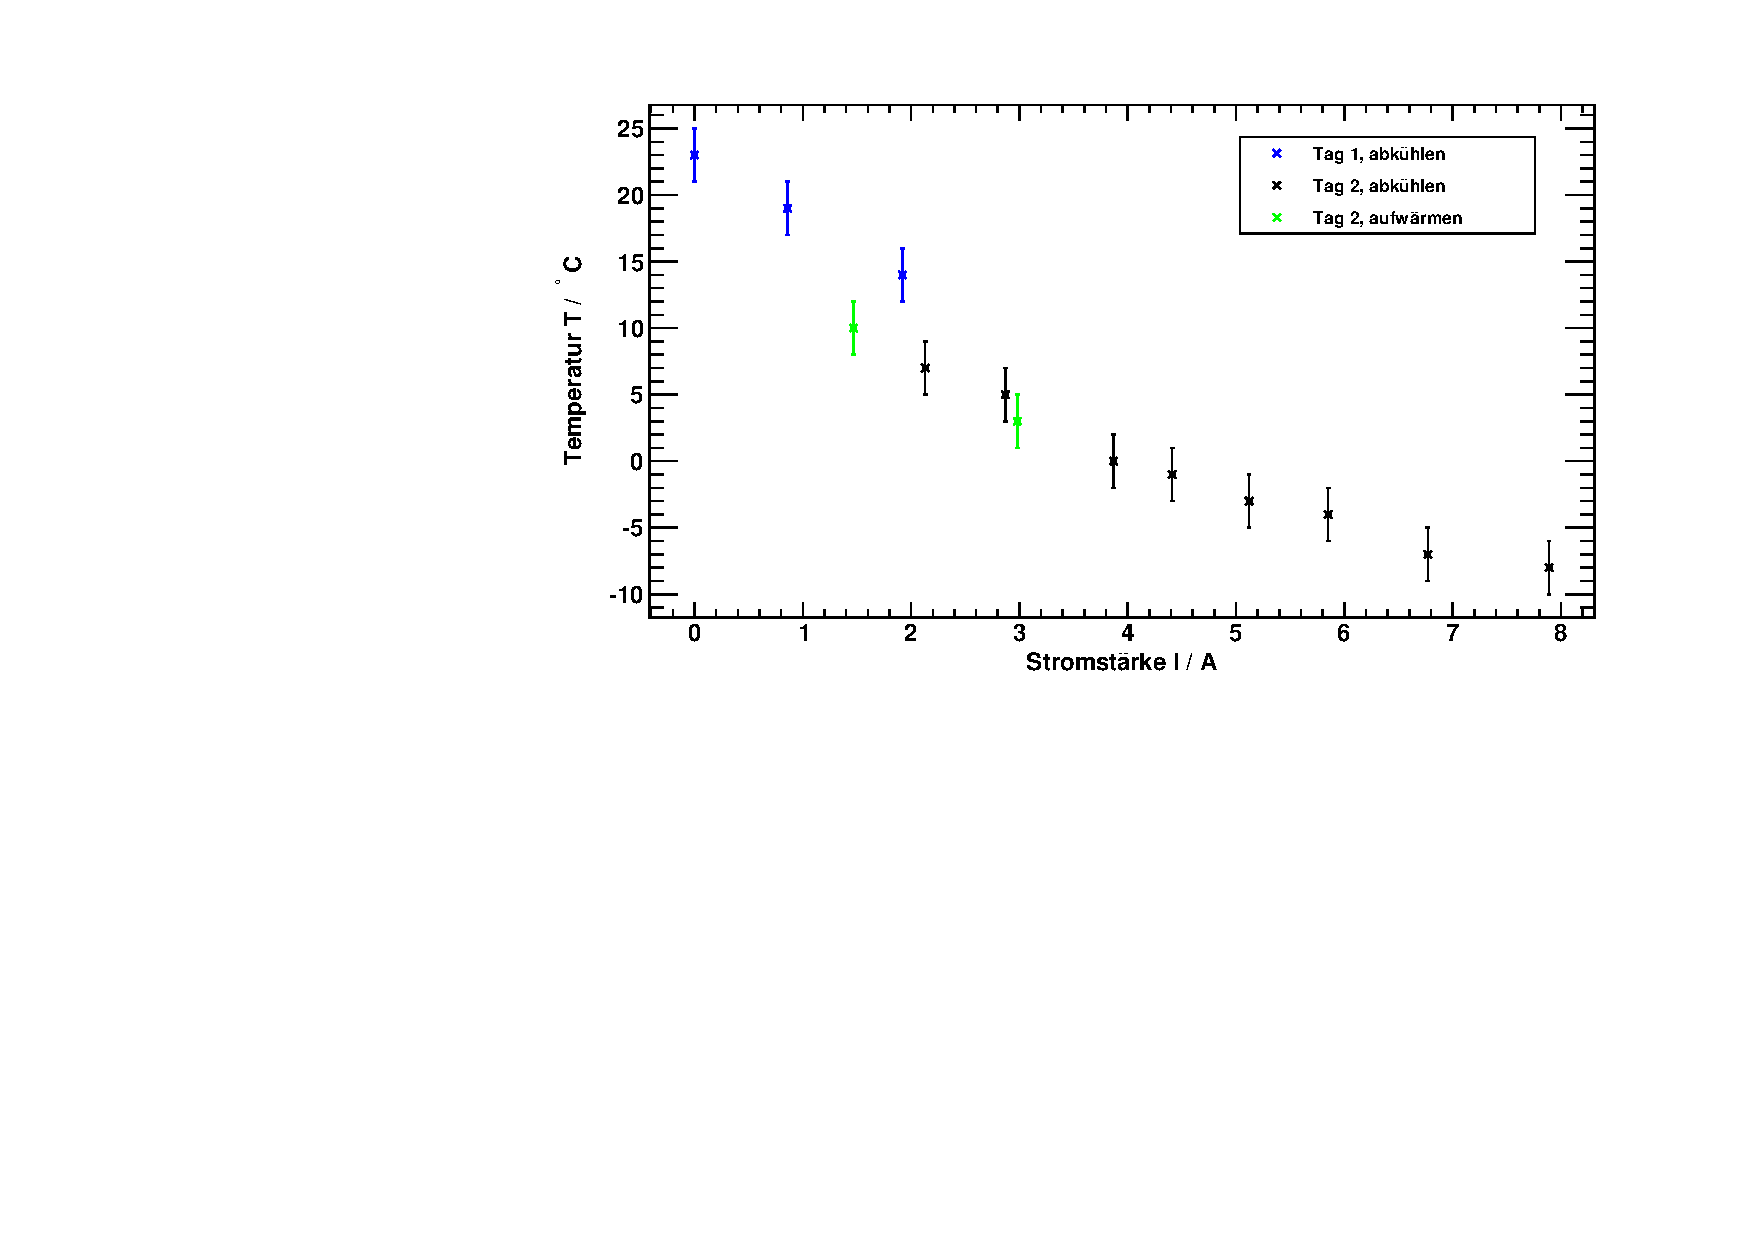
\includegraphics[width=\textwidth]{../img/graph_T-I.pdf}
  \caption{Temperatur am Thermoelement
  in Abhängigkeit des Stroms durch das Peltierelement.}
  \label{img:TI}
\end{center}
\end{figure}

\autoref{img:TI} zeigt den Zusammenhang zwischen Strom durch das Peltierelement
und der Temperatur, die sich nach 30 Minuten Stromfluss am Thermoelement eingestellt hat.
Es ist ein exponentieller Verlauf mit Sättigung bei hohem Strom zu erkennen.
Dies kann mit dem Wärmefluss aus der Umgebung begründet werden.
Auf einen Fit wurde hier verzichtet, da die genaue Information über den Zusammenhang
für die Auswertung nicht relevant ist.
Man erkennt allerdings, dass die Messwerte für Abkühlung (schwarz) und Erwärmung (grün) konsistent sind.
Die Einschwingzeit von 30 Minuten ist also lang genug gewählt.
Zwischen 1. und 2. Messtag besteht ein großer Offset.
Dies könnte an der Temperatur des Kühlwassers liegen,
das am ersten Tag von einem anderen Verbraucher im Haus erwärmt wurde.\\
\autoref{img:UI} zeigt die Strom-Spannungs-Kennlinie des Peltierelements.
Der Zusammenhang ist linear, der Widerstand beträgt über den gesamten Arbeitsbereich ca. 3\,\textOmega.
Die Kühlleistung des Elements ist also sowohl zum Quadrat des Stroms als auch zum Quadrat der Spannung proportional.



\begin{figure}[H]
\begin{center}
  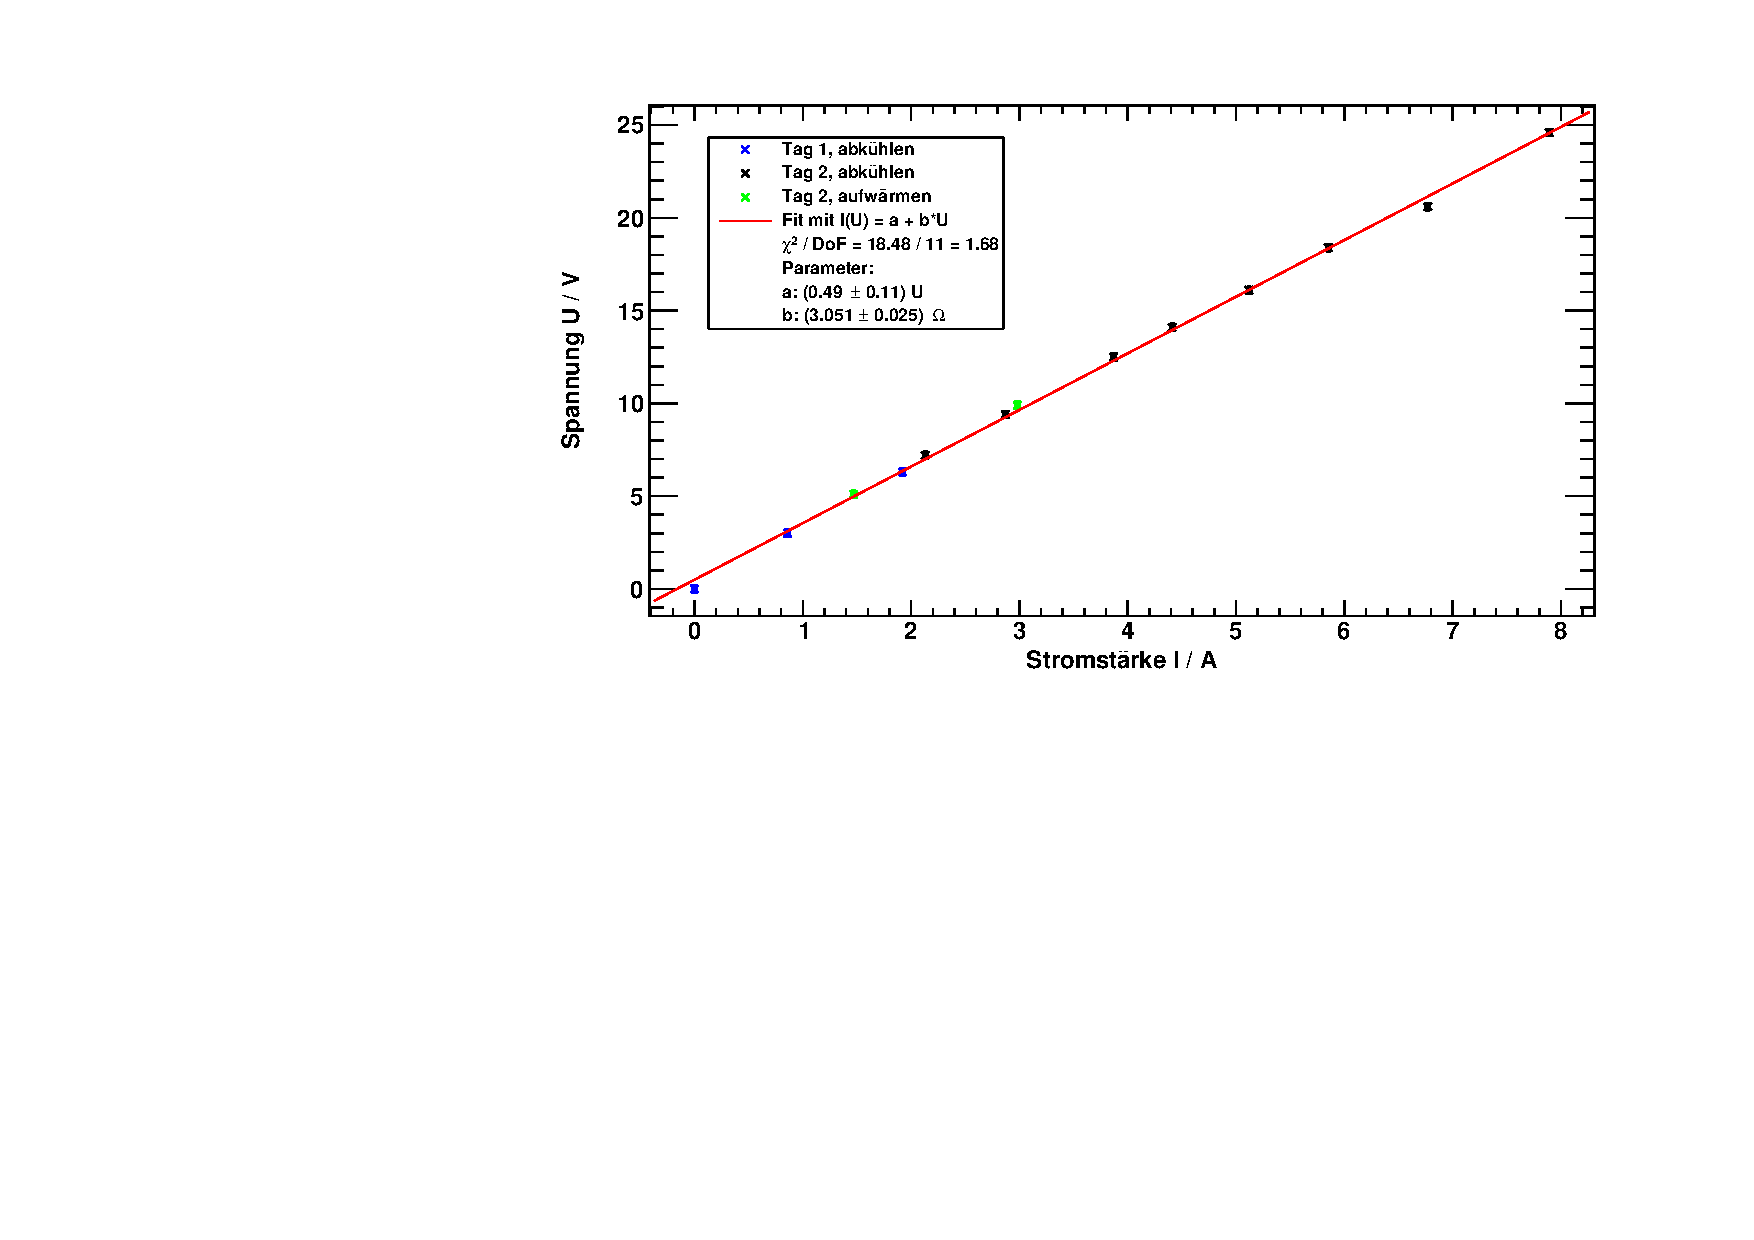
\includegraphics[width=\textwidth]{../img/graph_U-I.pdf}
  \caption{Strom-Spannungs-Kennlinie des Peltierelements.}
  \label{img:UI}
\end{center}
\end{figure}




\subsection{Bestimmung der Lebensdauer aus dem Lorentz-Peak}
\subsubsection{Vorgehensweise}
Für jede Messung erhält man zwei Graphen: Die Abhängigkeit der Rampenspannung $U$, die an der Spule anliegt, von der Zeit und der 
zeitliche Lorentzpeak des Hanle-Effekts. Die Spannung $U$ wird in dem Wertebereich, in dem sie sich verändert, mit 
einem Polynom ersten Grades gefittet (\autoref{img:fit:BV}). Der Fehler auf die Spannung $U$ und die Zeit $t$ wurde jeweils auf die Hälfte der 
Binbreite gesetzt.\footnote{Diese Werte werden hier nicht explizit angegeben, da sie für verschiedene Messungen aufgrund der unterschiedlichen 
Auflösung des Oszilloskops variieren.}
\begin{equation}
  \label{eq:BV:fitfunction}
  U(t) = a + b \cdot t
\end{equation}
\begin{figure}[H]
\begin{center}
  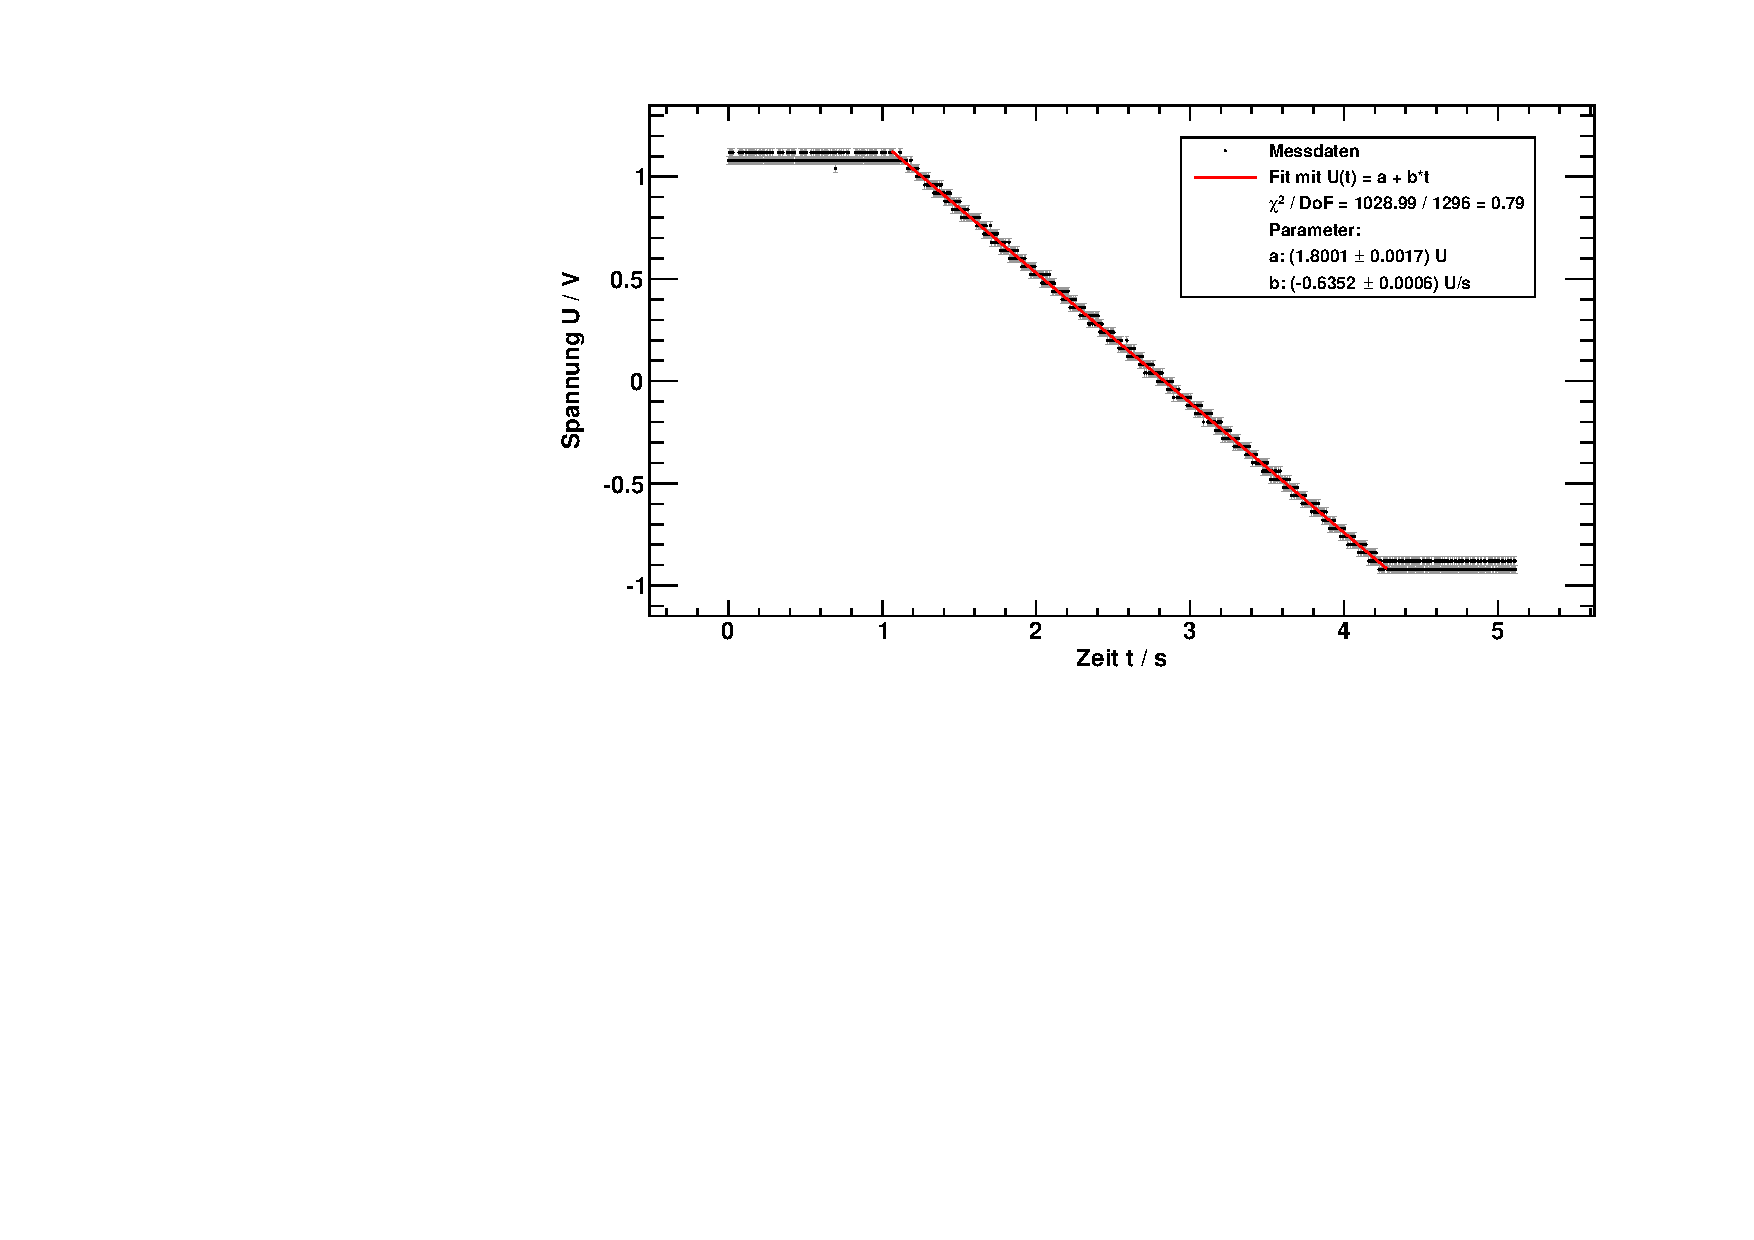
\includegraphics[width=\textwidth]{../img/fitBV_00_m03.pdf}
  \caption{Linearer Fit der angelegten Spannung $U$ an der Spule. Hier exemplarisch für $T=-3\,{}^\circ$C und $\Phi=0^\circ$.}
  \label{img:fit:BV}
\end{center}
\end{figure}
Da sich der Strom $I$, der durch Spule fließt, direkt aus dem Wert der Spannung $U$ ergibt ($I(t) = U(t) \cdot 1\,\frac{\text{A}}{\text{V}}$), kann man nun zu 
jedem Zeitpunkt $t$ (innerhalb der Änderung von $U$) die Stärke $B$ des angelegten Magnetfeldes bestimmen. Dazu benötigt man eine spulenspezifische 
Proportionalitätskonstante $p$, (hier $p=3.363\cdot10^{-4}\,\frac{\text{T}}{\text{A}}$), 
welche die Änderung des Flusses $B$ mit dem Strom $I$ beschreibt. 
Es folgt:
\begin{equation}
  B(t) = p \cdot I(t)
\end{equation}
Daraus lässt sich nun die Intensität des Hanle-Signals in Abhängigkeit des vorhandenen Magnetfeldes $B$ angeben (\autoref{img:fit:lorentz:0}, 
\autoref{img:fit:lorentz:45}, \autoref{img:fit:lorentz:90}).
Der Fehler auf das Magnetfeld wurde zu 1\% des Wertes gewählt. Auf die Intensität (hier gemessene Spannung $U$) wurde zusätzlich zur halben Binbreite 
noch ein relativer Fehler von $s_\text{rel} = 1\%$ des Messwerts gesetzt:
\begin{equation}
  s_U = \sqrt{s_{\text{Bin}}^2 + (s_\text{rel} \cdot U)^2}
\end{equation}
Dieser Graph kann nun mit \autoref{eq:intensity} gefittet werden.
\begin{figure}[H]
\begin{center}
  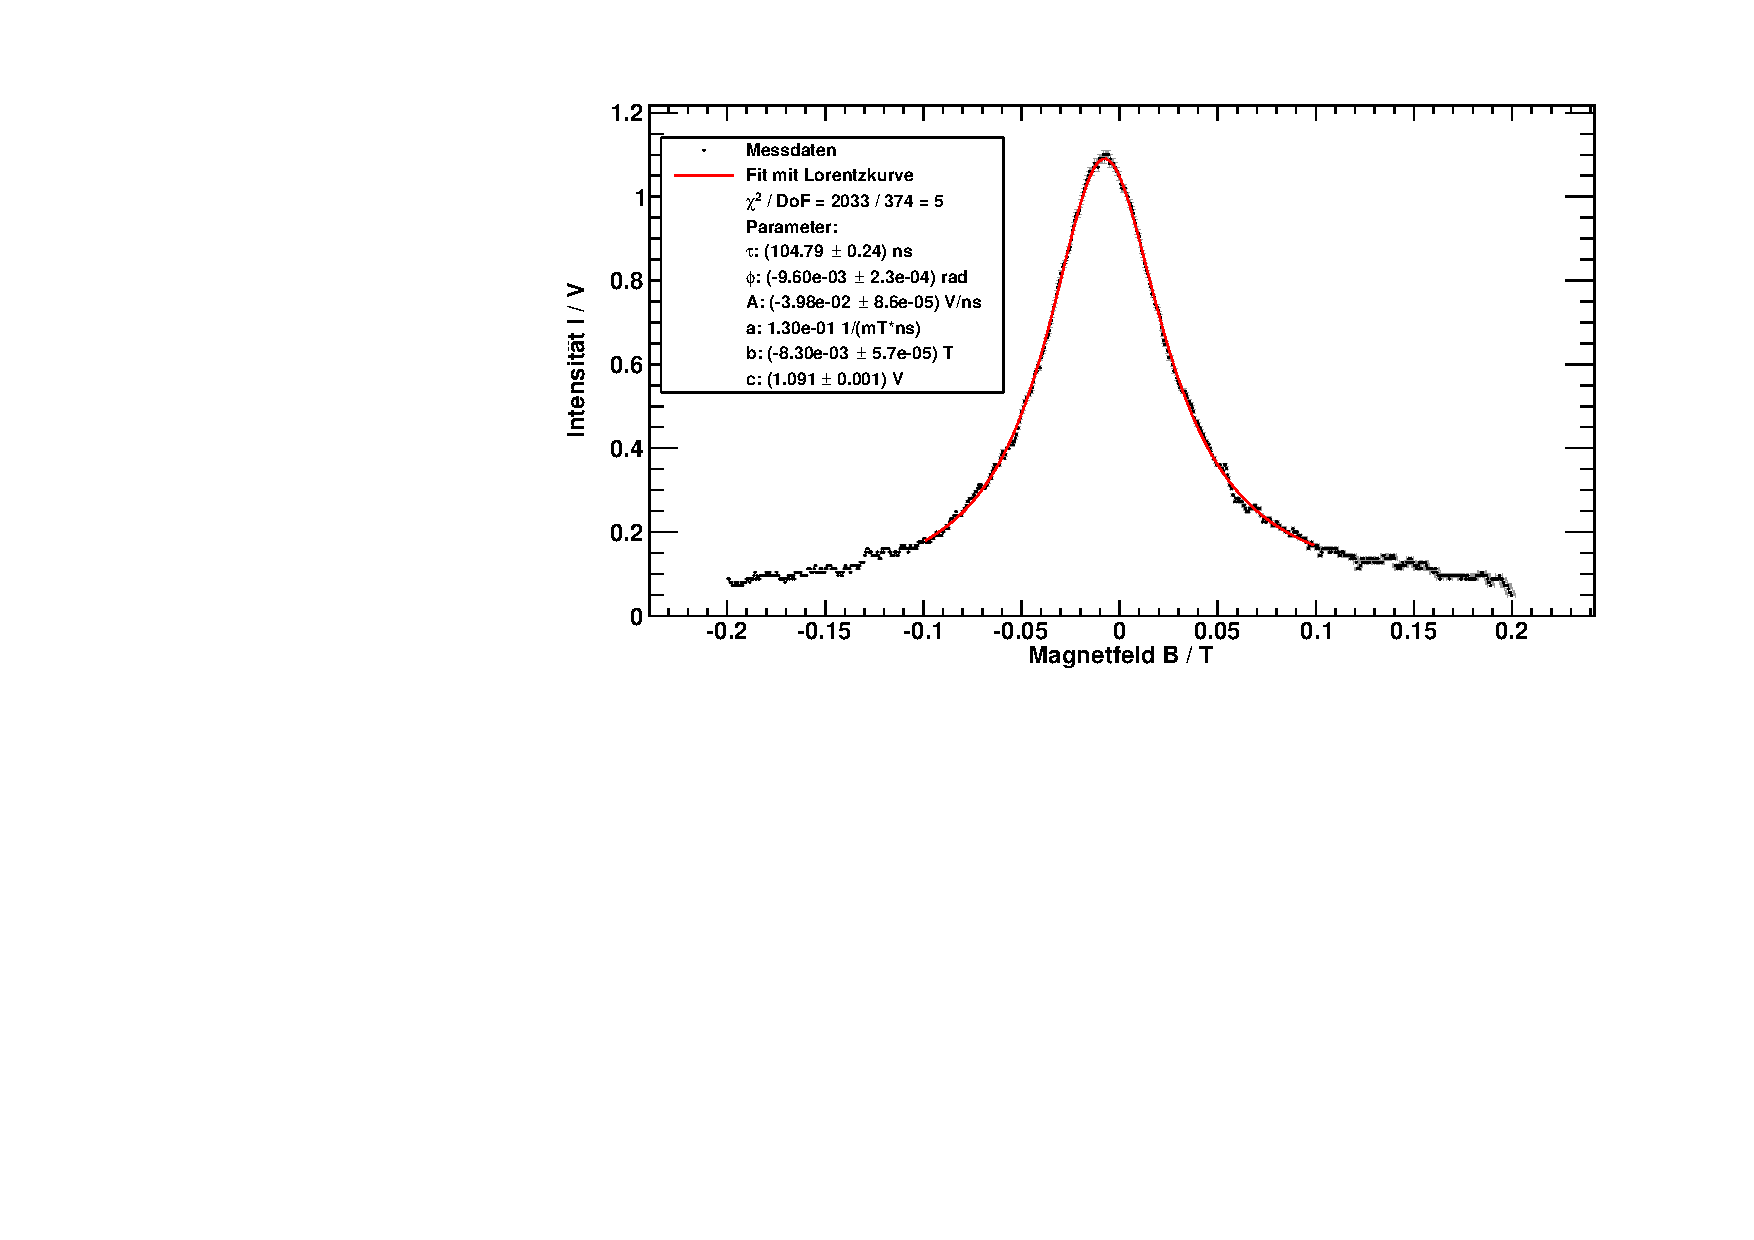
\includegraphics[width=\textwidth]{../img/fit_00_m03.pdf}
  \caption{Fit des Hanle-Signals mit Lorentzkurve. Hier exemplarisch für $T=-3\,{}^\circ$C und $\Phi=0^\circ$.}
  \label{img:fit:lorentz:0}
\end{center}
\end{figure}
\begin{figure}[H]
\begin{center}
  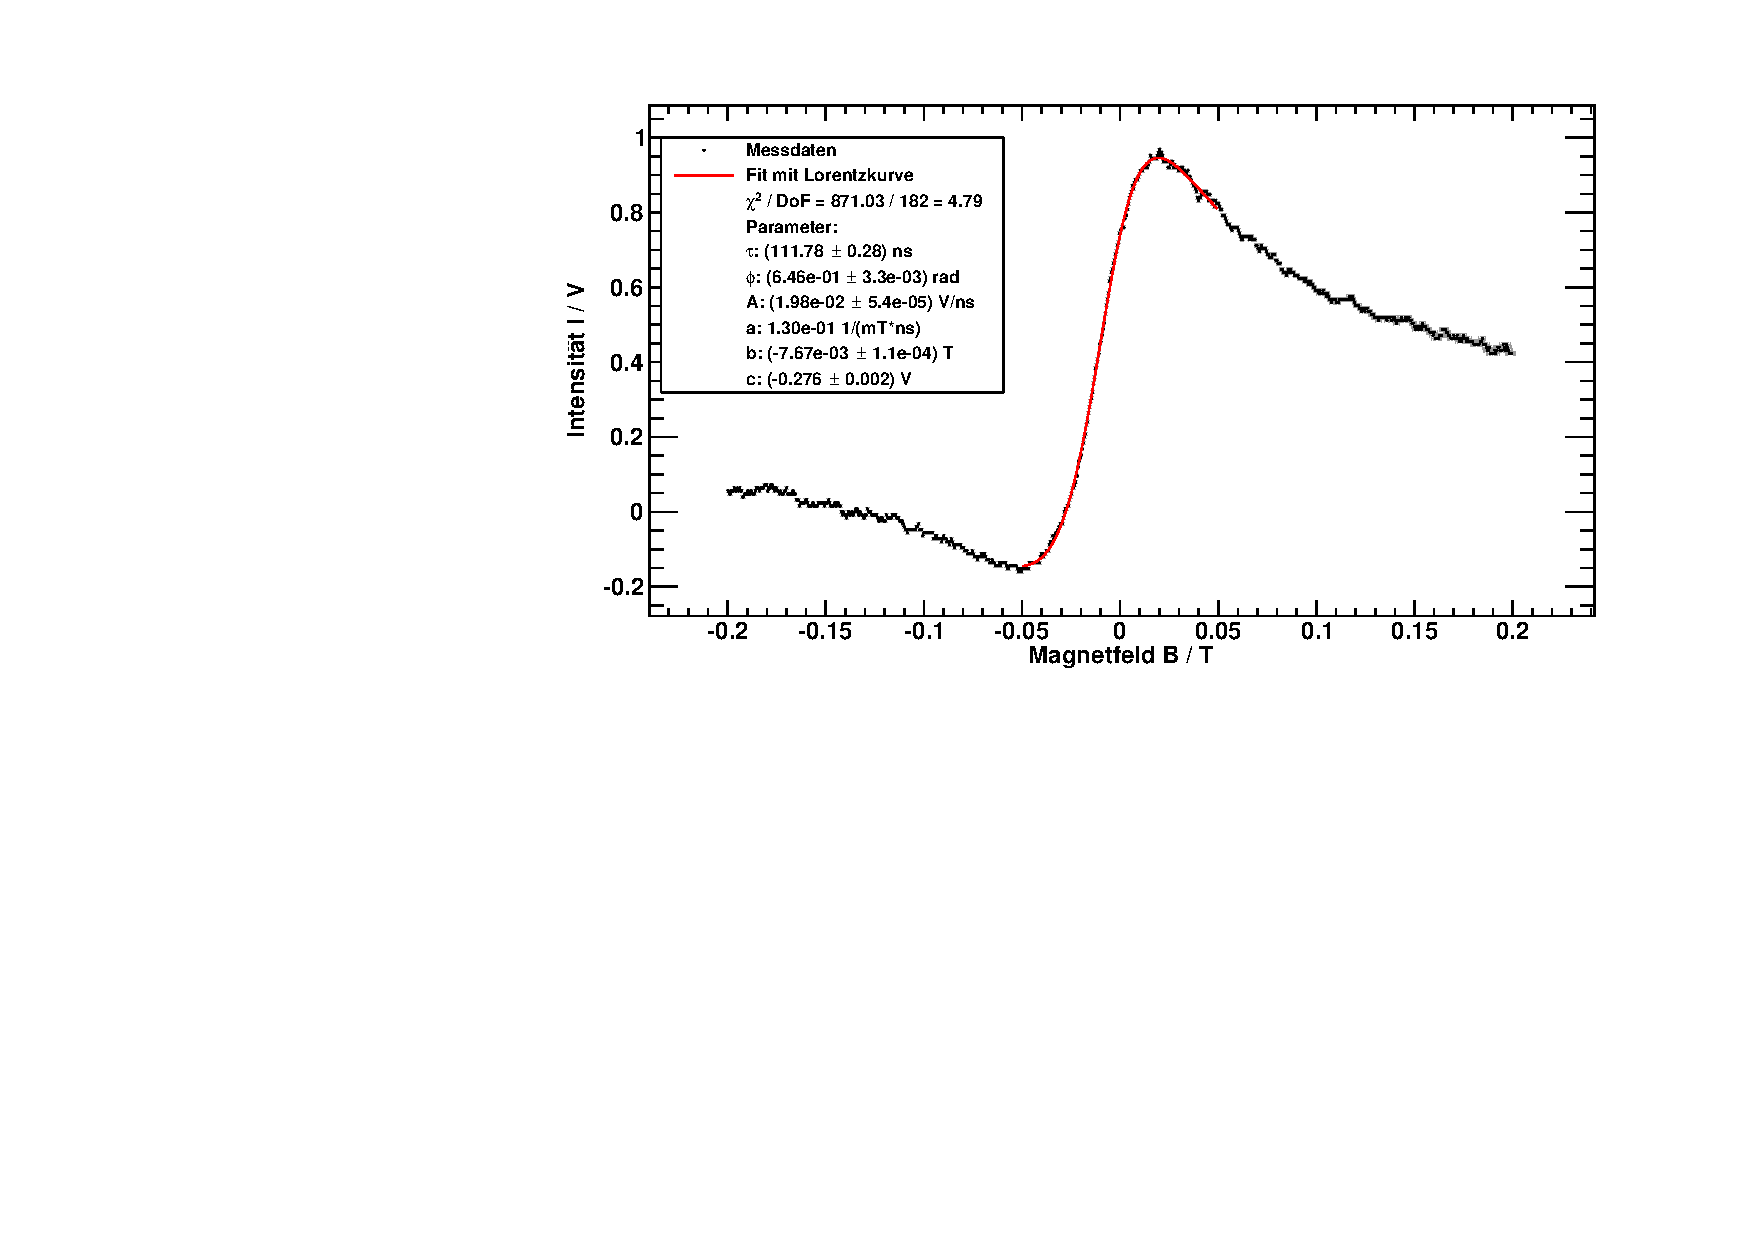
\includegraphics[width=\textwidth]{../img/fit_45_m03.pdf}
  \caption{Fit des Hanle-Signals mit Lorentzkurve. Hier exemplarisch für $T=-3\,{}^\circ$C und $\Phi=45^\circ$.}
  \label{img:fit:lorentz:45}
\end{center}
\end{figure}
\begin{figure}[H]
\begin{center}
  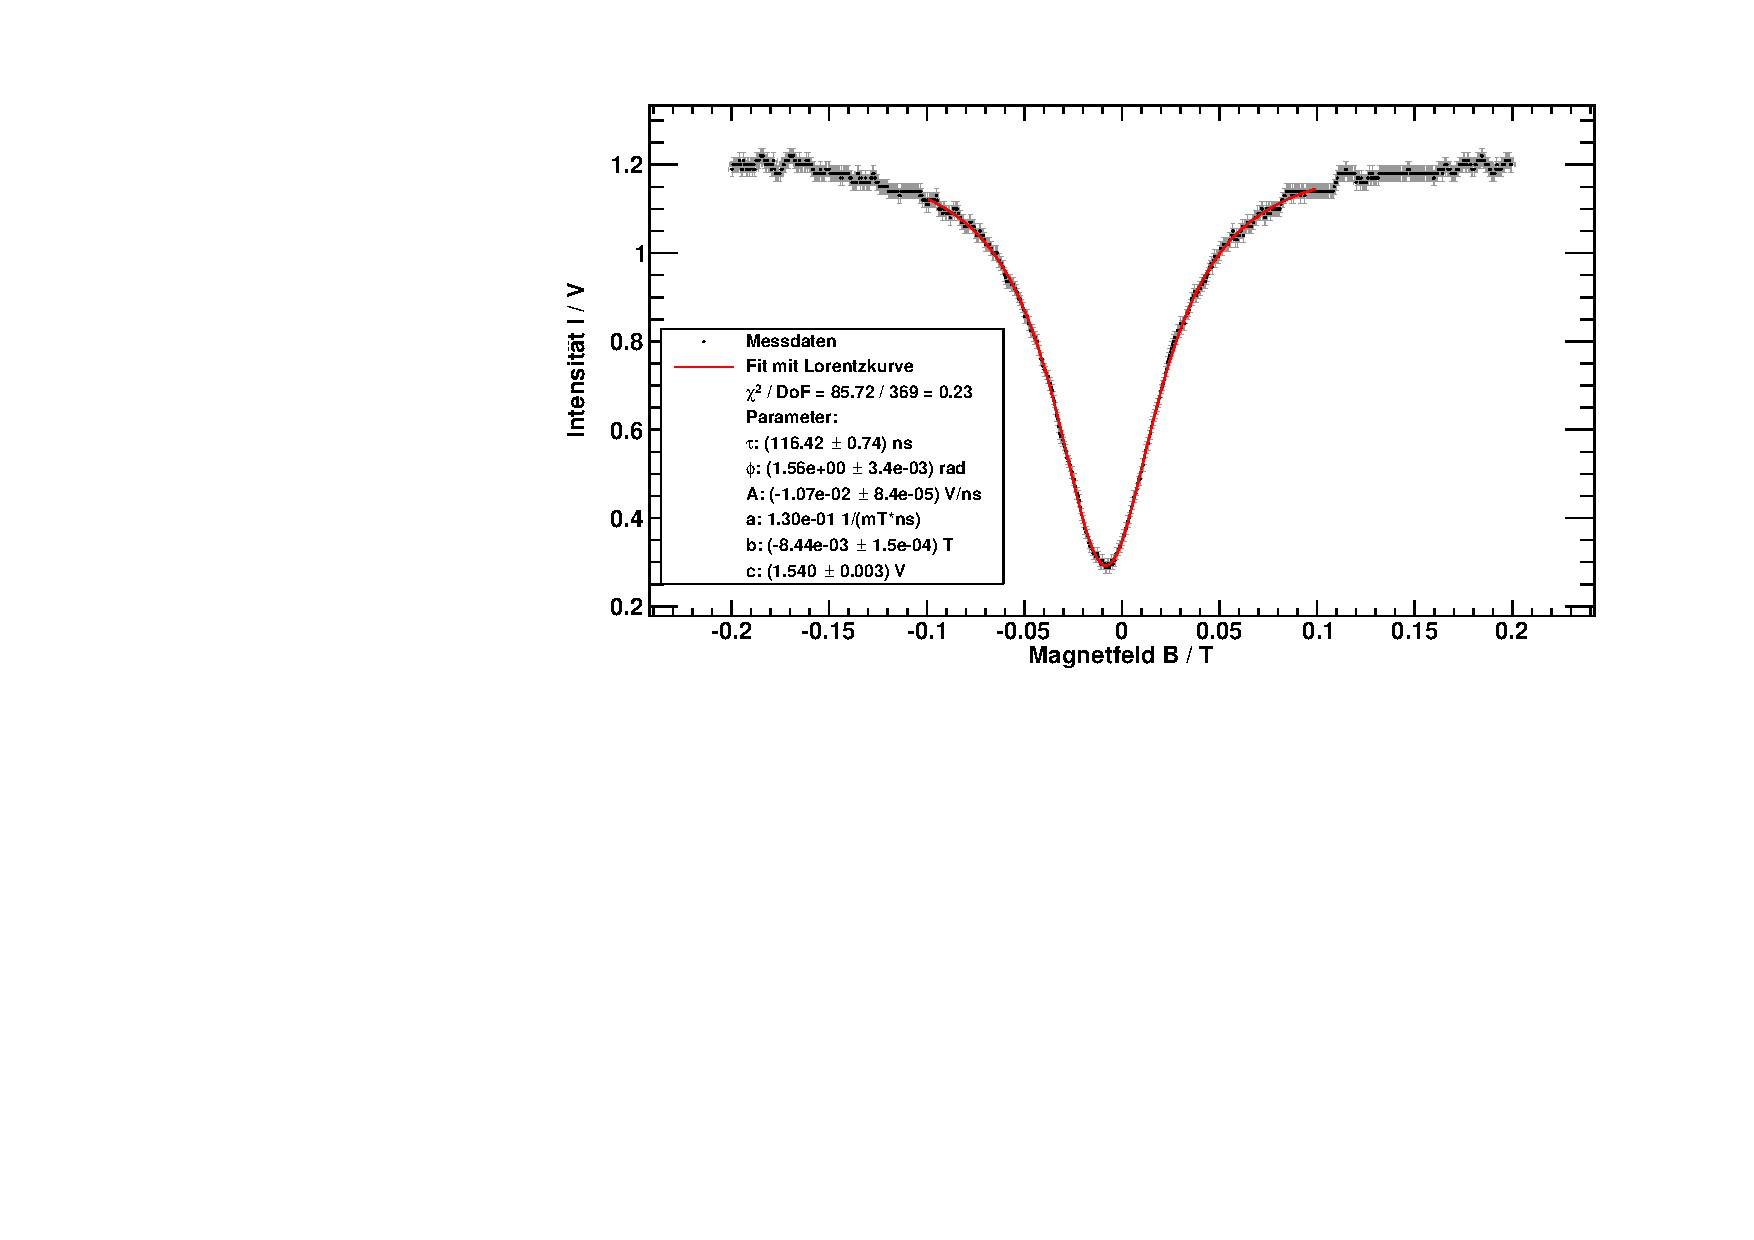
\includegraphics[width=\textwidth]{../img/fit_90_m03.pdf}
  \caption{Fit des Hanle-Signals mit Lorentzkurve. Hier exemplarisch für $T=-3\,{}^\circ$C und $\Phi=90^\circ$.}
  \label{img:fit:lorentz:90}
\end{center}
\end{figure}
Die Fitergebnisse aller Messungen werden in Abschnitt \ref{subsub:fitresults} diskutiert.

\subsubsection{Fehler auf die Lebensdauer}
\subsubsection{Fitergebnisse}
\label{subsub:fitresults}
\begin{table}[H]
\caption{Fitergebnisse f"ur $\Phi=0^\circ$.}
\begin{center}
\begin{tabular}{|c|c|c|c|c|}
  \hline
  $T$ / ${}^{\circ}$C & $\tau$ / ns & $s_{\tau}$ / ns & $\Phi$ / ${}^{\circ}$ & $s_{\Phi}$ / ${}^{\circ}$ \\ \hline
  23 & 124.9 & 1.6 & 0.648 & 0.032 \\ \hline
  19 & 122.1 & 1.5 & 0.906 & 0.029 \\ \hline
  14 & 122.9 & 1.5 & 0.041 & 0.025 \\ \hline
  10 & 116.1 & 1.5 & -0.447 & 0.019 \\ \hline
  7 & 122.9 & 1.5 & 0.219 & 0.020 \\ \hline
  5 & 116.6 & 1.5 & -0.056 & 0.139 \\ \hline
  3 & 111.7 & 1.4 & -0.238 & 0.020 \\ \hline
  0 & 110.4 & 1.4 & -0.288 & 0.020 \\ \hline
  -1 & 109.1 & 1.4 & -0.155 & 0.020 \\ \hline
  -3 & 104.2 & 1.3 & -0.538 & 0.025 \\ \hline
  -4 & 105.1 & 1.3 & -0.458 & 0.024 \\ \hline
  -7 & 102.2 & 1.3 & -0.476 & 0.029 \\ \hline
  -8 & 106.5 & 1.3 & -0.407 & 0.042 \\ \hline
\end{tabular}
\end{center}
\label{tab:phi:0}
\end{table}

\begin{table}[H]
\caption{Fitergebnisse f"ur $\varphi=45$}
\begin{center}
\begin{tabular}{|c|c|c|c|c|}
  \hline
  $T$ / ${}^{\circ}$C & $\tau$ / ns & $s_{\tau} / ns$ & $\varphi$ / ${}^{\circ}$ & $s_{\varphi}$ / ${}^{\circ}$ \\ \hline
  23 & 149.9 & 1.7 & 31.538 & 0.209 \\ \hline
  19 & 140.7 & 1.6 & 37.495 & 0.211 \\ \hline
  10 & 126.7 & 1.4 & 36.166 & 0.134 \\ \hline
  7 & 132.3 & 1.5 & 38.131 & 0.136 \\ \hline
  5 & 121.3 & 1.3 & 37.273 & 0.148 \\ \hline
  3 & 116.0 & 1.3 & 38.735 & 0.163 \\ \hline
  0 & 115.5 & 1.3 & 36.855 & 0.166 \\ \hline
  -1 & 120.6 & 1.3 & 35.438 & 0.156 \\ \hline
  -3 & 111.2 & 1.2 & 37.098 & 0.209 \\ \hline
  -4 & 111.2 & 1.2 & 35.342 & 0.222 \\ \hline
  -7 & 108.6 & 1.2 & 35.264 & 0.255 \\ \hline
  -8 & 104.6 & 1.2 & 38.696 & 0.331 \\ \hline
\end{tabular}
\end{center}
\label{tab:phi:45}
\end{table}

\begin{table}[H]
\caption{Fitergebnisse f"ur $\varphi=90$}
\begin{center}
\begin{tabular}{|c|c|c|c|c|}
  \hline
  $T$ / ${}^{\circ}$C & $\tau$ / ns & $s_{\tau} / ns$ & $\varphi$ / ${}^{\circ}$ & $s_{\varphi}$ / ${}^{\circ}$ \\ \hline
  23 & 160.5 & 1.7 & 88.197 & 0.095 \\ \hline
  19 & 164.0 & 1.8 & 89.482 & 0.087 \\ \hline
  10 & 134.6 & 1.4 & 95.995 & 0.049 \\ \hline
  7 & 134.8 & 1.4 & 95.089 & 0.053 \\ \hline
  5 & 131.0 & 1.4 & 96.695 & 0.499 \\ \hline
  3 & 123.9 & 1.3 & 97.930 & 0.054 \\ \hline
  0 & 126.2 & 1.4 & 97.914 & 0.054 \\ \hline
  -1 & 119.0 & 1.3 & 89.235 & 0.053 \\ \hline
  -3 & 116.3 & 1.2 & 89.605 & 0.059 \\ \hline
  -4 & 113.5 & 1.2 & 96.982 & 0.068 \\ \hline
  -7 & 110.3 & 1.2 & 97.656 & 0.076 \\ \hline
  -8 & 109.4 & 1.2 & 98.378 & 0.086 \\ \hline
\end{tabular}
\end{center}
\label{tab:phi:90}
\end{table}


\subsection{Extrapolation auf 0 Pa}